\section{Robustness of the storage results}\label{app:robust}

The tables and figures in this appendix back \cref{fig:readback,fig:patch}.
\Cref{tab:fig5-robust} recomputes the pooled patching shares when only forks with a gap of at least 0.1 are kept, % C21.32
when each problem is dropped in turn, and as a median over forks.
\Cref{tab:fig5-singles} gives the number vs number single layers that stand out, with Bonferroni-corrected lower
bounds over all 56 single-layer tests. % C21.35
\Cref{tab:fig5-nw} reports the number vs word blocks, whose gap is too small to localise.
\Cref{fig:readback-unbinned} shows the readback at single positions of the forced text, and \cref{fig:perfork} the
per-fork spread behind the pooled shares.

\begin{table*}[t]
\centering
\small
\caption{Robustness of the patching shares in Fig.~5. Pooled: share of the summed blend--control gap closed (as plotted). Gap $\geq$ 0.1: the same, keeping only forks whose gap is at least 0.1. Leave one out: range of the pooled share when each problem is dropped in turn. Median: median of per-fork shares over forks with gap $\geq$ 0.1. Fork probe, GSM8K items 10--49, 50/50 blends, forks where the model followed the chosen token.}
\label{tab:fig5-robust}
\begin{tabular}{lcccccccc}
\toprule
 & \multicolumn{4}{c}{Remove} & \multicolumn{4}{c}{Insert} \\
\cmidrule(lr){2-5} \cmidrule(lr){6-9}
Patched & Pooled & Gap $\geq$ 0.1 & Leave one out & Median & Pooled & Gap $\geq$ 0.1 & Leave one out & Median \\
\midrule
\multicolumn{9}{l}{\emph{Number vs number: 96 forks, 78 with gap $\geq$ 0.1}} \\
layers 0--3 & 0.58 & 0.56 & 0.56--0.62 & 0.53 & 0.55 & 0.54 & 0.54--0.59 & 0.49 \\
layers 4--7 & 0.19 & 0.19 & 0.18--0.20 & 0.16 & 0.16 & 0.16 & 0.14--0.17 & 0.10 \\
layers 8--11 & 0.06 & 0.06 & 0.05--0.06 & 0.02 & 0.09 & 0.09 & 0.08--0.10 & 0.04 \\
layers 12--15 & 0.12 & 0.10 & 0.11--0.12 & 0.06 & 0.17 & 0.16 & 0.15--0.18 & 0.10 \\
layer 0 & 0.38 & 0.36 & 0.35--0.41 & 0.12 & 0.16 & 0.16 & 0.14--0.17 & 0.02 \\
layer 1 & 0.21 & 0.20 & 0.19--0.22 & 0.14 & 0.07 & 0.07 & 0.06--0.08 & 0.05 \\
layer 2 & 0.20 & 0.19 & 0.19--0.22 & 0.12 & 0.05 & 0.06 & 0.05--0.06 & 0.03 \\
layer 7 & 0.13 & 0.13 & 0.12--0.13 & 0.11 & 0.12 & 0.12 & 0.11--0.13 & 0.06 \\
layer 13 & 0.08 & 0.07 & 0.07--0.09 & 0.04 & 0.13 & 0.12 & 0.12--0.14 & 0.05 \\
\addlinespace
\multicolumn{9}{l}{\emph{Word vs word: 139 forks, 108 with gap $\geq$ 0.1}} \\
layers 0--3 & 0.66 & 0.63 & 0.65--0.69 & 0.66 & 0.75 & 0.72 & 0.73--0.77 & 0.78 \\
layers 4--7 & 0.10 & 0.10 & 0.10--0.11 & 0.09 & 0.16 & 0.16 & 0.15--0.17 & 0.15 \\
layers 8--11 & 0.04 & 0.05 & 0.04--0.04 & 0.03 & 0.07 & 0.07 & 0.06--0.07 & 0.06 \\
layers 12--15 & 0.03 & 0.04 & 0.03--0.04 & 0.02 & 0.06 & 0.06 & 0.05--0.06 & 0.05 \\
\bottomrule
\end{tabular}
\end{table*}

\begin{table}[t]
\centering
\small
\caption{Number vs number single layers that stand out in Figure~5c. 95\% CI: bootstrap over problems (2,000 resamples). Corrected lower: lower bound of the Bonferroni-corrected interval for all 56 single-layer tests (28 layers $\times$ remove/insert; 20,000 resamples). Every bound is above 0. The single-layer analysis was not pre-registered.}
\label{tab:fig5-singles}
\begin{tabular}{lcccccc}
\toprule
 & \multicolumn{3}{c}{Remove} & \multicolumn{3}{c}{Insert} \\
\cmidrule(lr){2-4} \cmidrule(lr){5-7}
Patched & Share & 95\% CI & Corrected lower & Share & 95\% CI & Corrected lower \\
\midrule
layer 0 & 0.38 & [0.27, 0.50] & 0.20 & 0.16 & [0.10, 0.23] & 0.06 \\
layer 1 & 0.21 & [0.15, 0.27] & 0.12 & 0.07 & [0.03, 0.10] & 0.01 \\
layer 2 & 0.20 & [0.15, 0.26] & 0.12 & 0.05 & [0.03, 0.08] & 0.01 \\
layer 7 & 0.13 & [0.10, 0.16] & 0.08 & 0.12 & [0.08, 0.17] & 0.05 \\
layer 13 & 0.08 & [0.05, 0.12] & 0.04 & 0.13 & [0.09, 0.17] & 0.06 \\
\bottomrule
\end{tabular}
\end{table}

\begin{table*}[t]
\centering
\small
\caption{Number vs word forks (34 forks from 21 problems), not shown in Fig.~5. The mean blend--control gap is only 0.11, so the shares are unstable (wide CIs, values above 1 and below 0) and cannot localise the runner-up. 95\% CI: bootstrap over problems.}
\label{tab:fig5-nw}
\begin{tabular}{lcccc}
\toprule
 & \multicolumn{2}{c}{Remove} & \multicolumn{2}{c}{Insert} \\
\cmidrule(lr){2-3} \cmidrule(lr){4-5}
Patched & Share & 95\% CI & Share & 95\% CI \\
\midrule
layers 0--3 & 0.98 & [0.63, 2.31] & 0.90 & [0.67, 1.55] \\
layers 4--7 & 0.11 & [0.02, 0.59] & $-$0.01 & [$-$0.24, 0.11] \\
layers 8--11 & $-$0.01 & [$-$0.10, 0.02] & 0.00 & [$-$0.09, 0.06] \\
layers 12--15 & $-$0.03 & [$-$0.12, 0.01] & $-$0.02 & [$-$0.25, 0.05] \\
layers 16--19 & 0.14 & [0.00, 0.38] & 0.08 & [$-$0.03, 0.21] \\
layers 20--23 & 0.07 & [$-$0.01, 0.20] & $-$0.01 & [$-$0.11, 0.05] \\
layers 24--27 & 0.04 & [$-$0.14, 0.12] & 0.03 & [$-$0.09, 0.10] \\
\bottomrule
\end{tabular}
\end{table*}


\begin{figure}[t]
\centering
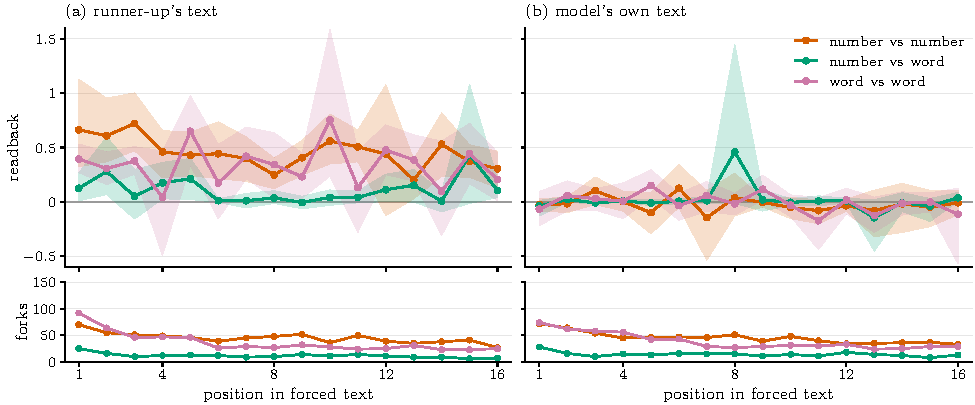
\includegraphics{figA1.pdf}
\caption{Readback at each position of the forced text, without the binning of \cref{fig:readback}b--c.
Top: mean readback (control minus blend) with 95\% bootstrap CIs over problems, for the runner-up's text
(left) and the model's own text (right).
Bottom: number of forks with a defined score at that position (positions where the chosen token and the runner-up
barely differ are skipped).
With the runner-up's text, the mean stays above 0 at every position for number vs number and word vs word; % C21.38
with the model's own text it stays around 0.
Single positions hold few forks, so their CIs are wide; this is why \cref{fig:readback} pools positions into
log-spaced bins.}
\label{fig:readback-unbinned}
\end{figure}

\begin{figure}[t]
\centering
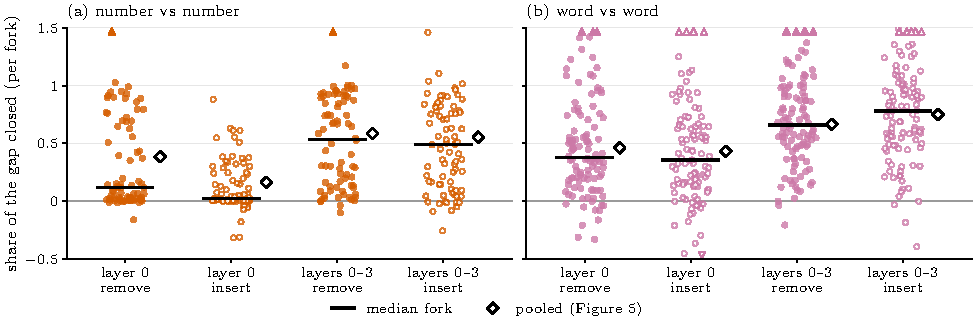
\includegraphics{figA2.pdf}
\caption{Per-fork shares behind the pooled bars of \cref{fig:patch}, for layer 0 and layers 0--3. % C21.31
Each dot is one fork with a blend--control gap of at least 0.1 % C21.32
(78 number vs number forks, 108 word vs word); % C21.32
filled = remove, open = insert.
Black bar: median per fork.
Diamond: pooled share, as plotted in \cref{fig:patch}.
For number vs number, layer 0 is uneven across forks: half of them have a remove
share below 0.12 and a quarter are above 0.68, % C21.39
so the pooled 0.38 sits well above the median fork % C21.34
(0.12; insert: 0.16 vs 0.02). % C21.34
For layers 0--3 the median fork is close to the pooled share. % C21.31
Dots outside the axis range are drawn at its edge as triangles.}
\label{fig:perfork}
\end{figure}
